% TikZ scaffold; panels in Figures/exp_frames/ are crops of the old
% 2d_nav_figure.png -- regenerate from matplotlib with the paper palette
% (seal RGB 0,140,90; glide RGB 200,120,0; tli RGB 80,80,80) for print quality.
\begin{tikzpicture}[font=\small,
  photo/.style={inner sep=0pt}, lbl/.style={font=\scriptsize, align=center}]
\node[photo] (a) {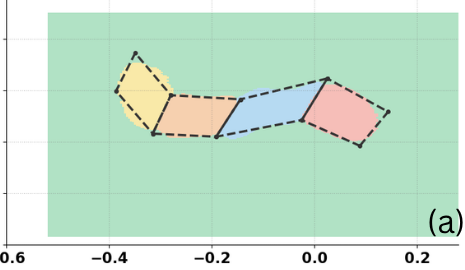
\includegraphics[height=3.0cm]{Figures/exp_frames/nav_guards.png}};
\node[photo, right=4mm of a] (b) {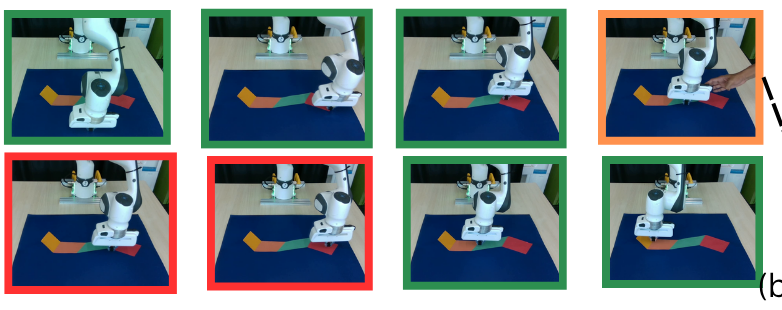
\includegraphics[height=3.0cm]{Figures/exp_frames/nav_episode.png}};
\node[photo, right=4mm of b] (c) {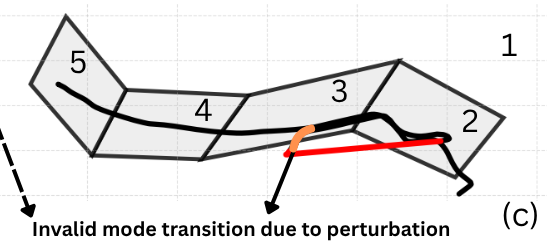
\includegraphics[height=3.0cm]{Figures/exp_frames/nav_traj.png}};
\node[lbl, below=1mm of a] {(a) learned guards (dashed)\\ vs.\ ground-truth regions};
\node[lbl, below=1mm of b] {(b) hardware episode: perturbation\\ (orange frame) and recovery (red frames)};
\node[lbl, below=1mm of c] {(c) executed trajectory over modes;\\ \textcolor{red}{red} = recovery segment};
\end{tikzpicture}
